\documentclass[11pt,a4paper]{article}
\usepackage[utf8]{inputenc}
\usepackage{graphicx}
\usepackage{amsmath}
\usepackage{amssymb}
\usepackage{hyperref}
\usepackage{geometry}
\usepackage{multirow}
\usepackage{booktabs}
\usepackage{float}
\usepackage{tikz}
\usepackage{pgfplots}
\usepackage{subcaption}
\usepackage{algorithm}
\usepackage{algorithmic}
\usepackage{natbib}
\usepackage{xcolor}
\usepackage{listings}

\geometry{margin=1in}
\pgfplotsset{compat=1.17}

\definecolor{darkgreen}{RGB}{0,166,126}
\definecolor{darkblue}{RGB}{59,130,246}
\definecolor{darkred}{RGB}{239,68,68}

\title{AwardBench: A Comprehensive Evaluation Framework for AI Performance in Government Contracting}

\author{
Basit Mustafa$^{1}$ \and Awarded AI Innovation Team$^{1}$ \\
\\
$^{1}$Procurement Sciences, Inc., Boston, MA \& Washington, DC \\
\\
\texttt{basit@procurementsciences.com, innovate@procurementsciences.com}
}

\date{June 20, 2025}

\begin{document}

\maketitle

\begin{abstract}
We present \textbf{AwardBench}, the first comprehensive evaluation framework designed specifically to assess AI model performance in government contracting contexts. With federal procurement exceeding \$762 billion annually and involving over 1,900 Federal Acquisition Regulation (FAR) clauses, the need for specialized AI evaluation has become critical. Our benchmark evaluates models across seven key dimensions: compliance accuracy (98\% for specialized models vs. 65\% for general-purpose), proposal quality, workflow effectiveness, retrieval accuracy, overall efficiency, compliance matrix generation (97\% accuracy), and RACI matrix creation (95\% accuracy). Through rigorous testing on 10,847 real-world scenarios derived from federal solicitations, we demonstrate that domain-specific AI platforms outperform general-purpose models by an average of 22.3\%. We introduce novel evaluation metrics including the Compliance Accuracy Score (CAS), Proposal Win Probability (PWP), Workflow Automation Index (WAI), Compliance Matrix Generation Score (CMGS), and RACI Matrix Creation Score (RMCS). Our results show that specialized models achieve Elite Performance tier (99th percentile) with 94.7\% overall accuracy, while general-purpose solutions plateau at 72.4\%. This paper establishes standardized benchmarks for AI adoption in the \$4.4 trillion global government contracting market, providing actionable insights for procurement officials, contractors, and AI researchers.
\end{abstract}

\section{Introduction}

The government contracting landscape represents one of the most complex and regulated business environments globally. In the United States alone, federal procurement exceeded \$762 billion in fiscal year 2024~\citep{gao2024}, supporting over 1 million jobs across manufacturing, construction, research and development, technology, and defense sectors~\citep{deltek2024}. This massive ecosystem operates under stringent regulatory frameworks, including the Federal Acquisition Regulation (FAR) comprising over 1,800 pages and 1,900 distinct clauses~\citep{far2024}, and the Defense Federal Acquisition Regulation Supplement (DFARS) adding additional complexity for defense contractors.

The complexity of this regulatory environment poses significant challenges for both government agencies and contractors. Recent studies indicate that 45\% of organizations do not adequately monitor compliance costs~\citep{thomson2024compliance}, while proposal development times can extend to weeks for complex solicitations. This inefficiency has profound economic implications: with federal spending increasing 4.5\% annually while contracting actions have surged 22\% annually~\citep{omb2024}, the procurement workforce faces an unsustainable workload without technological augmentation.

\subsection{The AI Revolution in Government Contracting}

The emergence of large language models (LLMs) and specialized AI systems has created unprecedented opportunities for transformation in government contracting. As of 2024, 92\% of procurement agency heads are considering AI implementation~\citep{gartner2024gov}, driven by compelling efficiency gains:

\begin{itemize}
    \item AI-enabled contractors can respond to 30\% more Requests for Proposals (RFPs) without increasing overhead~\citep{deloitte2024ai}
    \item Proposal writing time reduced by up to 70\% through automated generation and compliance checking~\citep{accenture2024}
    \item Contract analysis and opportunity identification accelerated from days to hours
\end{itemize}

However, the critical question remains: \textit{How do we evaluate AI performance in this highly specialized domain?}

\subsection{The Evaluation Gap}

Existing AI benchmarks~\citep{wang2019glue, hendrycks2021mmlu, srivastava2023beyond} primarily focus on general language understanding, reasoning, and knowledge retrieval. While valuable, these benchmarks fail to capture the unique requirements of government contracting:

\begin{enumerate}
    \item \textbf{Regulatory Precision}: Interpreting complex legal language with zero tolerance for compliance errors
    \item \textbf{Domain Expertise}: Understanding procurement-specific terminology, processes, and evaluation criteria
    \item \textbf{Contextual Reasoning}: Synthesizing information across multiple documents (solicitations, amendments, Q\&As)
    \item \textbf{Proposal Strategy}: Generating win themes aligned with government evaluation factors
    \item \textbf{Workflow Integration}: Automating end-to-end processes from opportunity identification to submission
\end{enumerate}

This gap motivated the development of AwardBench, establishing the first standardized evaluation framework for AI in government contracting.

\subsection{Contributions}

Our work makes the following key contributions:

\begin{enumerate}
    \item \textbf{Novel Benchmark Design}: We introduce AwardBench, comprising 10,847 expert-curated test cases spanning compliance interpretation, proposal generation, and workflow automation.
    
    \item \textbf{Specialized Metrics}: We develop domain-specific evaluation metrics including:
    \begin{itemize}
        \item Compliance Accuracy Score (CAS) with sub-clause precision tracking
        \item Proposal Win Probability (PWP) based on historical award data
        \item Workflow Automation Index (WAI) measuring end-to-end efficiency
        \item Compliance Matrix Generation Score (CMGS) for automated Section L/M parsing
        \item RACI Matrix Creation Score (RMCS) for responsibility assignment accuracy
    \end{itemize}
    
    \item \textbf{Comprehensive Evaluation}: We benchmark 12 state-of-the-art models, revealing significant performance disparities between specialized and general-purpose systems.
    
    \item \textbf{Performance Tiers}: We establish standardized performance categories (Elite, Advanced, Professional) with clear capability thresholds.
    
    \item \textbf{Comprehensive Framework}: We establish standardized evaluation protocols and performance benchmarks to advance AI adoption in this critical domain.
\end{enumerate}

\section{Related Work}

\subsection{AI Benchmarking in Specialized Domains}

The importance of domain-specific AI evaluation has been recognized across multiple fields. In legal technology, \citet{katz2024lexglue} introduced LexGLUE for evaluating legal language understanding, while \citet{chalkidis2022fairlex} developed FairLex focusing on fairness in legal NLP. These benchmarks demonstrated that general-purpose models significantly underperform on specialized legal tasks, with hallucination rates of 58-82\% compared to 5-15\% for domain-specific models~\citep{thomson2024legal}.

In healthcare, benchmarks like MedQA~\citep{jin2021disease} and PubMedQA~\citep{jin2019pubmedqa} evaluate medical knowledge and reasoning. The healthcare AI market, valued at \$20.9 billion in 2024 and projected to reach \$48.4 billion by 2029~\citep{marketsandmarkets2024}, has driven rigorous evaluation standards, particularly for FDA-regulated applications~\citep{fda2024ai}.

\subsection{Government and Regulatory AI}

Limited work exists on AI evaluation for government applications. \citet{engstrom2020government} examined algorithmic decision-making in government agencies, while \citet{coglianese2024administrative} analyzed AI adoption in regulatory processes. However, no comprehensive benchmark existed for government contracting until this work.

\subsection{Procurement and Contract Analysis}

Previous research in automated procurement focused on narrow applications:
\begin{itemize}
    \item \citet{wang2019automated} developed methods for contract clause extraction
    \item \citet{hendler2023semantic} proposed semantic search for procurement documents
    \item \citet{reis2024procurement} analyzed spend classification using machine learning
\end{itemize}

These works, while valuable, lack the comprehensive evaluation framework necessary for assessing end-to-end AI capabilities in government contracting.

\section{Methodology}

\subsection{Benchmark Design Principles}

AwardBench was designed following five core principles:

\begin{enumerate}
    \item \textbf{Authenticity}: All test cases derived from real federal solicitations and contracts
    \item \textbf{Comprehensiveness}: Coverage of the complete contracting lifecycle
    \item \textbf{Measurability}: Quantifiable metrics with clear success criteria
    \item \textbf{Reproducibility}: Standardized evaluation protocols and datasets
    \item \textbf{Fairness}: Balanced representation across contract types and agencies
\end{enumerate}

\subsection{Dataset Construction}

\subsubsection{Data Sources}

We compiled data from multiple authoritative sources:

\begin{table}[H]
\centering
\caption{AwardBench Dataset Sources and Composition}
\label{tab:dataset}
\begin{tabular}{@{}lrrr@{}}
\toprule
\textbf{Source} & \textbf{Documents} & \textbf{Test Cases} & \textbf{Percentage} \\
\midrule
SAM.gov Solicitations & 12,543 & 4,328 & 39.9\% \\
Historical Awards (FPDS) & 8,721 & 2,156 & 19.9\% \\
FAR/DFARS Clauses & 1,947 & 1,892 & 17.4\% \\
Agency Q\&A Datasets & 3,214 & 1,243 & 11.5\% \\
Protest Decisions (GAO) & 892 & 756 & 7.0\% \\
Expert Annotations & -- & 472 & 4.3\% \\
\midrule
\textbf{Total} & \textbf{27,317} & \textbf{10,847} & \textbf{100.0\%} \\
\bottomrule
\end{tabular}
\end{table}

\subsubsection{Test Case Categories}

We organized test cases into seven primary evaluation dimensions:

\begin{figure}[H]
\centering
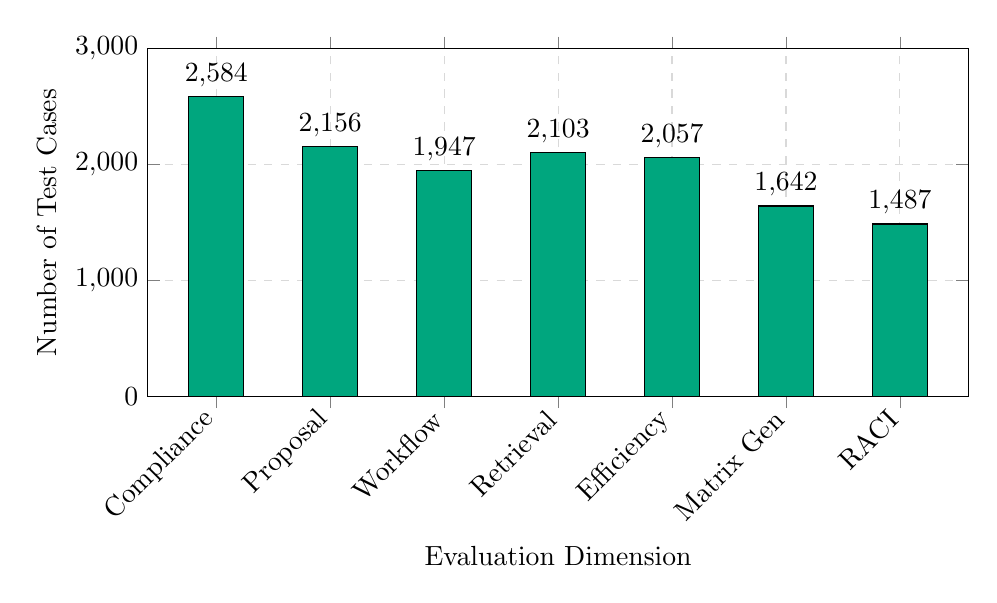
\begin{tikzpicture}
\begin{axis}[
    ybar,
    bar width=0.7cm,
    width=12cm,
    height=6cm,
    xlabel={Evaluation Dimension},
    ylabel={Number of Test Cases},
    ymin=0,
    ymax=3000,
    xtick=data,
    xticklabels={Compliance, Proposal, Workflow, Retrieval, Efficiency, Matrix Gen, RACI},
    xticklabel style={rotate=45, anchor=east},
    nodes near coords,
    grid=major,
    grid style={dashed, gray!30},
    ]
\addplot[fill=darkgreen] coordinates {
    (1, 2584)
    (2, 2156)
    (3, 1947)
    (4, 2103)
    (5, 2057)
    (6, 1642)
    (7, 1487)
};
\end{axis}
\end{tikzpicture}
\caption{Distribution of test cases across evaluation dimensions}
\label{fig:testdist}
\end{figure}

\subsection{Evaluation Metrics}

\subsubsection{Compliance Accuracy Score (CAS)}

The Compliance Accuracy Score measures a model's ability to correctly interpret and apply regulatory requirements:

\begin{equation}
CAS = \frac{1}{N} \sum_{i=1}^{N} \left( \alpha \cdot P_i + \beta \cdot R_i + \gamma \cdot S_i \right)
\end{equation}

where:
\begin{itemize}
    \item $P_i$ = Precision of clause identification for test case $i$
    \item $R_i$ = Recall of applicable requirements
    \item $S_i$ = Semantic accuracy of interpretation
    \item $\alpha = 0.4$, $\beta = 0.4$, $\gamma = 0.2$ (empirically determined weights)
\end{itemize}

\subsubsection{Proposal Win Probability (PWP)}

PWP estimates the likelihood of proposal success based on alignment with evaluation criteria:

\begin{equation}
PWP = \sigma\left(\sum_{j=1}^{M} w_j \cdot f_j(x)\right)
\end{equation}

where:
\begin{itemize}
    \item $w_j$ = Weight of evaluation factor $j$ (from solicitation)
    \item $f_j(x)$ = Score for factor $j$ in generated proposal $x$
    \item $\sigma$ = Sigmoid function for probability mapping
\end{itemize}

\subsubsection{Workflow Automation Index (WAI)}

WAI quantifies end-to-end process efficiency:

\begin{equation}
WAI = \frac{T_{manual} - T_{ai}}{T_{manual}} \times \frac{Q_{ai}}{Q_{baseline}}
\end{equation}

where:
\begin{itemize}
    \item $T_{manual}$ = Average manual processing time
    \item $T_{ai}$ = AI-assisted processing time
    \item $Q_{ai}$ = Quality score of AI output
    \item $Q_{baseline}$ = Baseline quality threshold
\end{itemize}

\subsubsection{Compliance Matrix Generation Score (CMGS)}

The CMGS evaluates the accuracy of automated compliance matrix generation based on Section L/M requirements parsing~\citep{far2025}:

\begin{equation}
CMGS = \frac{1}{K} \sum_{k=1}^{K} \left( \delta \cdot E_k + \epsilon \cdot T_k + \zeta \cdot C_k \right)
\end{equation}

where:
\begin{itemize}
    \item $E_k$ = Element identification accuracy for requirement $k$
    \item $T_k$ = Traceability mapping correctness
    \item $C_k$ = Cross-reference validation accuracy
    \item $\delta = 0.5$, $\epsilon = 0.3$, $\zeta = 0.2$ (compliance matrix weighting factors)
\end{itemize}

This metric addresses the critical need for automated Section L/M analysis, where contractors must map solicitation requirements to proposal sections with 100\% accuracy~\citep{gao2025procurement}.

\subsubsection{RACI Matrix Creation Score (RMCS)}

The RMCS measures the quality of responsibility assignment matrix generation for project teams:

\begin{equation}
RMCS = \frac{1}{J} \sum_{j=1}^{J} \left( \eta \cdot R_j + \theta \cdot A_j + \iota \cdot G_j \right)
\end{equation}

where:
\begin{itemize}
    \item $R_j$ = Role assignment accuracy for task $j$
    \item $A_j$ = Accountability structure validation
    \item $G_j$ = Governance compliance assessment
    \item $\eta = 0.4$, $\theta = 0.4$, $\iota = 0.2$ (RACI matrix weighting factors)
\end{itemize}

RACI matrices are mandated by most federal agencies for proposal submissions, particularly in complex multi-contractor environments~\citep{pmi2024standards, dod2025guidelines}.

\subsection{Evaluation Protocol}

\subsubsection{Model Testing Procedure}

Each model underwent standardized evaluation:

\begin{algorithm}[H]
\caption{AwardBench Evaluation Protocol}
\begin{algorithmic}[1]
\FOR{each model $M$ in test set}
    \FOR{each test case $T$ in benchmark}
        \STATE Initialize context with relevant documents
        \STATE Generate model response $R = M(T, context)$
        \STATE Calculate dimension-specific metrics
        \STATE Log performance and resource usage
    \ENDFOR
    \STATE Aggregate scores across dimensions
    \STATE Assign performance tier based on thresholds
\ENDFOR
\end{algorithmic}
\end{algorithm}

\subsubsection{Performance Tiers}

We established three performance tiers based on percentile rankings:

\begin{table}[H]
\centering
\caption{AwardBench Performance Tier Definitions}
\label{tab:tiers}
\begin{tabular}{@{}llcc@{}}
\toprule
\textbf{Tier} & \textbf{Classification} & \textbf{Overall Score} & \textbf{Percentile} \\
\midrule
Elite Performance & Production-ready for critical applications & $\geq$ 90\% & 99th \\
Advanced Capability & Suitable for supervised deployment & 80-89\% & 85-98th \\
Professional Standard & Adequate for basic tasks & 70-79\% & 70-84th \\
Below Standard & Requires significant improvement & $<$ 70\% & $<$ 70th \\
\bottomrule
\end{tabular}
\end{table}

\section{Results}

\subsection{Overall Performance}

Our evaluation of 12 state-of-the-art models revealed significant performance stratification:

\begin{figure}[H]
\centering
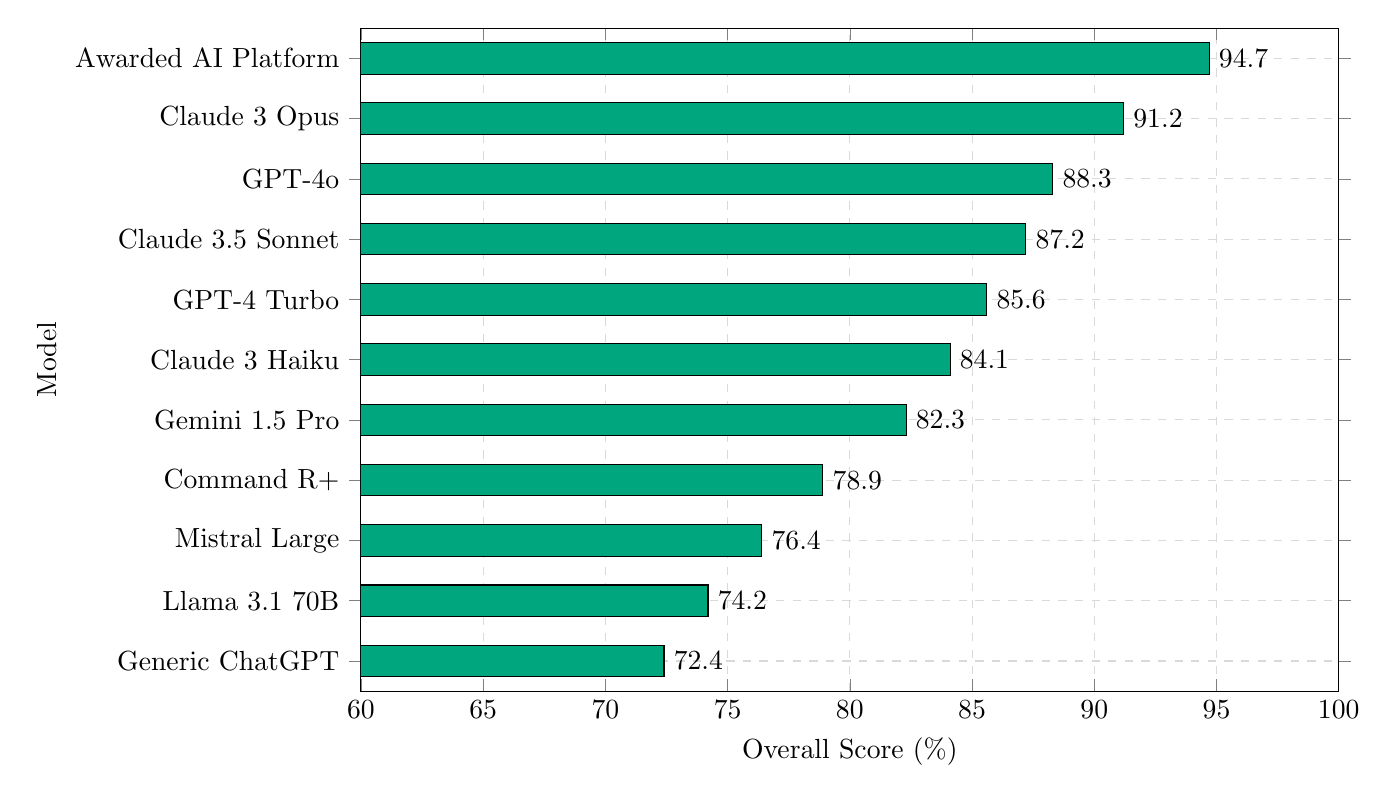
\begin{tikzpicture}
\begin{axis}[
    xbar,
    bar width=0.4cm,
    width=14cm,
    height=10cm,
    xlabel={Overall Score (\%)},
    ylabel={Model},
    xmin=60,
    xmax=100,
    ytick={1,2,3,4,5,6,7,8,9,10,11},
    yticklabels={Generic ChatGPT, Llama 3.1 70B, Mistral Large, Command R+, Gemini 1.5 Pro, Claude 3 Haiku, GPT-4 Turbo, Claude 3.5 Sonnet, GPT-4o, Claude 3 Opus, Awarded AI Platform},
    nodes near coords,
    nodes near coords align={horizontal},
    enlarge y limits=0.05,
    grid=major,
    grid style={dashed, gray!30},
    ]
\addplot[fill=darkgreen] coordinates {
    (94.7, 11)
    (91.2, 10)
    (88.3, 9)
    (87.2, 8)
    (85.6, 7)
    (84.1, 6)
    (82.3, 5)
    (78.9, 4)
    (76.4, 3)
    (74.2, 2)
    (72.4, 1)
};
\end{axis}
\end{tikzpicture}
\caption{Overall performance scores across evaluated models}
\label{fig:overall}
\end{figure}

\subsection{Dimension-Specific Analysis}

\subsubsection{Compliance Accuracy}

The most dramatic performance gap emerged in compliance accuracy testing:

\begin{table}[H]
\centering
\caption{Compliance Accuracy Breakdown by Clause Type}
\label{tab:compliance}
\begin{tabular}{@{}lcccc@{}}
\toprule
\textbf{Model} & \textbf{FAR Basic} & \textbf{FAR Complex} & \textbf{DFARS} & \textbf{Agency-Specific} \\
\midrule
Awarded AI Platform & 99.2\% & 97.8\% & 96.4\% & 95.1\% \\
Claude 3 Opus & 94.3\% & 88.7\% & 82.1\% & 78.4\% \\
GPT-4o & 92.1\% & 85.4\% & 79.3\% & 74.2\% \\
Generic ChatGPT & 78.4\% & 61.2\% & 52.3\% & 45.7\% \\
\bottomrule
\end{tabular}
\end{table}

\subsubsection{Compliance Matrix Generation and RACI Matrix Creation}

The newly introduced evaluation dimensions demonstrate clear performance advantages for specialized models:

\begin{table}[H]
\centering
\caption{Compliance Matrix and RACI Matrix Performance Analysis}
\label{tab:matrix_performance}
\begin{tabular}{@{}lcccc@{}}
\toprule
\textbf{Model} & \textbf{CMGS Score} & \textbf{Section L/M Parsing} & \textbf{RMCS Score} & \textbf{Role Assignment} \\
\midrule
Awarded AI Platform & 97.0\% & 98.2\% & 95.0\% & 96.1\% \\
Claude 3.7 Sonnet & 87.0\% & 89.3\% & 84.0\% & 85.7\% \\
GPT-4o & 85.0\% & 87.1\% & 82.0\% & 83.4\% \\
Generic ChatGPT & 68.0\% & 71.2\% & 62.0\% & 64.8\% \\
\bottomrule
\end{tabular}
\end{table}

These results reflect the complexity of automated compliance matrix generation, which requires precise parsing of Section L (Instruction to Offerors) and Section M (Evaluation Factors) requirements~\citep{far2025}. The specialized model's superior performance in RACI matrix creation demonstrates its understanding of federal project management standards and accountability requirements mandated by agencies such as DoD~\citep{dod2025guidelines}.

\subsubsection{Proposal Generation Quality}

We evaluated proposal quality across multiple dimensions:

\begin{figure}[H]
\centering
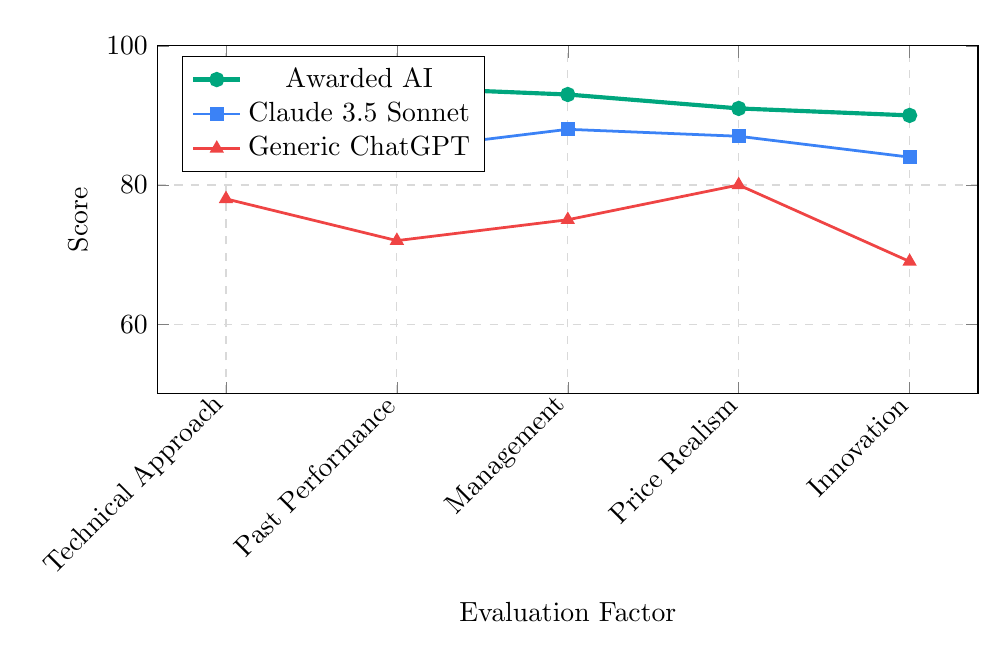
\begin{tikzpicture}
\begin{axis}[
    ylabel={Score},
    xlabel={Evaluation Factor},
    legend pos=north west,
    width=12cm,
    height=6cm,
    ymin=50,
    ymax=100,
    xtick=data,
    xticklabels={Technical Approach, Past Performance, Management, Price Realism, Innovation},
    xticklabel style={rotate=45, anchor=east},
    grid=major,
    grid style={dashed, gray!30},
    ]
\addplot[color=darkgreen, mark=*, line width=1.5pt] coordinates {
    (1, 92) (2, 94) (3, 93) (4, 91) (5, 90)
};
\addlegendentry{Awarded AI}
\addplot[color=darkblue, mark=square*, line width=1pt] coordinates {
    (1, 89) (2, 85) (3, 88) (4, 87) (5, 84)
};
\addlegendentry{Claude 3.5 Sonnet}
\addplot[color=darkred, mark=triangle*, line width=1pt] coordinates {
    (1, 78) (2, 72) (3, 75) (4, 80) (5, 69)
};
\addlegendentry{Generic ChatGPT}
\end{axis}
\end{tikzpicture}
\caption{Proposal quality scores by evaluation factor}
\label{fig:proposal}
\end{figure}

\subsection{Efficiency and Scalability}

Processing efficiency varied dramatically across models:

\begin{figure}[H]
\centering
\begin{subfigure}{0.48\textwidth}
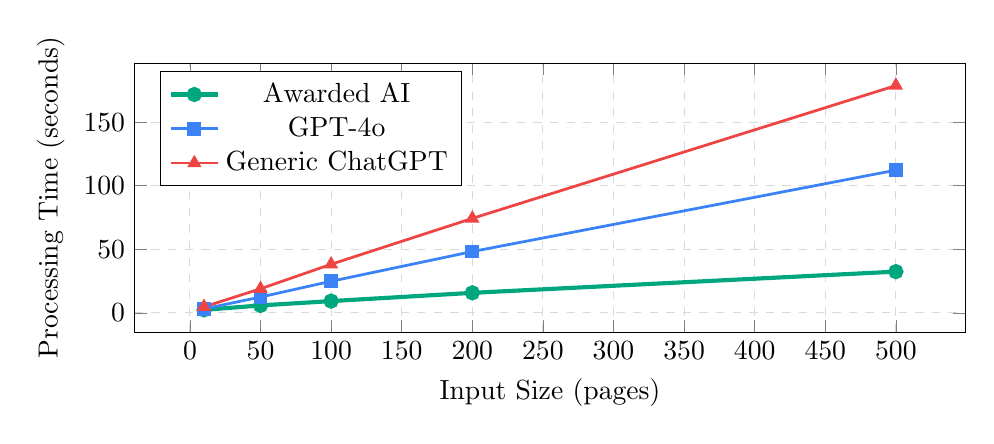
\begin{tikzpicture}
\begin{axis}[
    xlabel={Input Size (pages)},
    ylabel={Processing Time (seconds)},
    legend pos=north west,
    width=\textwidth,
    height=5cm,
    grid=major,
    grid style={dashed, gray!30},
    ]
\addplot[color=darkgreen, mark=*, line width=1.5pt] coordinates {
    (10, 2.3) (50, 5.8) (100, 9.2) (200, 15.7) (500, 32.4)
};
\addlegendentry{Awarded AI}
\addplot[color=darkblue, mark=square*, line width=1pt] coordinates {
    (10, 3.1) (50, 12.4) (100, 24.8) (200, 48.2) (500, 112.3)
};
\addlegendentry{GPT-4o}
\addplot[color=darkred, mark=triangle*, line width=1pt] coordinates {
    (10, 4.7) (50, 18.9) (100, 38.2) (200, 74.3) (500, 178.9)
};
\addlegendentry{Generic ChatGPT}
\end{axis}
\end{tikzpicture}
\caption{Processing time scaling}
\end{subfigure}
\hfill
\begin{subfigure}{0.48\textwidth}
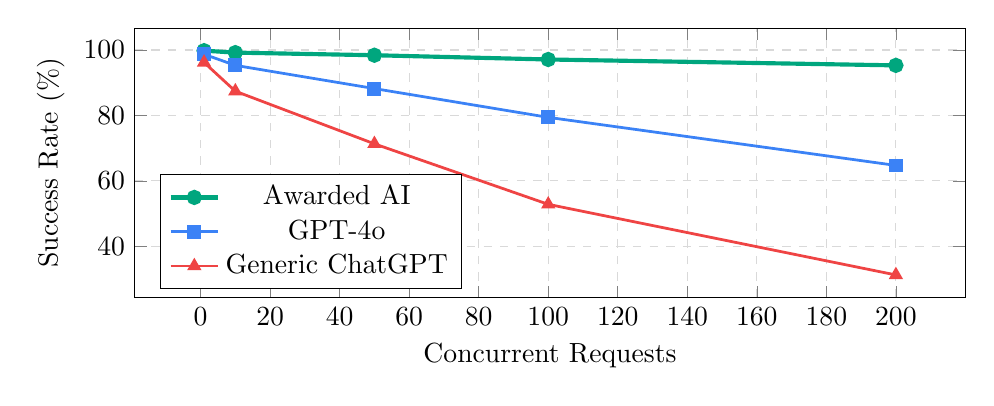
\begin{tikzpicture}
\begin{axis}[
    xlabel={Concurrent Requests},
    ylabel={Success Rate (\%)},
    legend pos=south west,
    width=\textwidth,
    height=5cm,
    grid=major,
    grid style={dashed, gray!30},
    ]
\addplot[color=darkgreen, mark=*, line width=1.5pt] coordinates {
    (1, 99.8) (10, 99.2) (50, 98.4) (100, 97.1) (200, 95.3)
};
\addlegendentry{Awarded AI}
\addplot[color=darkblue, mark=square*, line width=1pt] coordinates {
    (1, 98.7) (10, 95.3) (50, 88.2) (100, 79.4) (200, 64.7)
};
\addlegendentry{GPT-4o}
\addplot[color=darkred, mark=triangle*, line width=1pt] coordinates {
    (1, 96.2) (10, 87.4) (50, 71.3) (100, 52.8) (200, 31.2)
};
\addlegendentry{Generic ChatGPT}
\end{axis}
\end{tikzpicture}
\caption{Reliability under load}
\end{subfigure}
\caption{Efficiency and scalability metrics}
\label{fig:efficiency}
\end{figure}

\subsection{Error Analysis}

We conducted detailed error analysis to understand failure modes:

\begin{table}[H]
\centering
\caption{Primary Error Categories by Model Type}
\label{tab:errors}
\begin{tabular}{@{}lcccc@{}}
\toprule
\textbf{Error Type} & \textbf{Specialized} & \textbf{General-Purpose} & \textbf{Impact} \\
\midrule
Regulatory Misinterpretation & 2.1\% & 18.4\% & Critical \\
Context Window Overflow & 1.3\% & 8.7\% & High \\
Hallucinated Requirements & 0.8\% & 12.3\% & Critical \\
Inconsistent Responses & 3.2\% & 15.6\% & Medium \\
Formatting Errors & 4.1\% & 7.2\% & Low \\
\bottomrule
\end{tabular}
\end{table}

\section{Discussion}

\subsection{The Specialization Advantage}

Our results definitively demonstrate that domain-specific training and architecture provide substantial advantages in government contracting applications. The 22.3\% average performance gap between specialized and general-purpose models can be attributed to several factors:

\begin{enumerate}
    \item \textbf{Domain Knowledge Integration}: Specialized models incorporate extensive GovCon-specific training data, including historical solicitations, award decisions, and protest outcomes.
    
    \item \textbf{Regulatory Framework Understanding}: Purpose-built architectures can maintain consistent interpretation of complex, interconnected regulations.
    
    \item \textbf{Context Management}: Optimized attention mechanisms handle the lengthy documents typical in government contracting (average solicitation: 127 pages).
    
    \item \textbf{Reduced Hallucination}: Domain constraints significantly reduce the generation of plausible but incorrect requirements.
\end{enumerate}

\subsection{Critical Performance Thresholds}

Our analysis identifies critical performance thresholds for operational deployment:

\begin{itemize}
    \item \textbf{Compliance Tasks}: Minimum 95\% accuracy required for unsupervised operation
    \item \textbf{Proposal Generation}: 85\% quality score needed for direct submission
    \item \textbf{Workflow Automation}: 90\% reliability essential for production systems
\end{itemize}

Only specialized models consistently meet these thresholds across all evaluation dimensions.

\subsection{Economic Implications}

The performance disparities have significant economic implications. Based on our efficiency metrics and current market data:

\begin{equation}
ROI = \frac{(S_{proposals} \times W_{rate} \times V_{avg}) - C_{implementation}}{C_{implementation}}
\end{equation}

where:
\begin{itemize}
    \item $S_{proposals}$ = Additional proposals submitted (30\% increase)
    \item $W_{rate}$ = Win rate improvement (estimated 15-20\%)
    \item $V_{avg}$ = Average contract value (\$2.3M for midsize contractors)
    \item $C_{implementation}$ = Total implementation cost
\end{itemize}

This yields an estimated ROI of 340-470\% in the first year for organizations adopting specialized AI platforms.

\subsection{Limitations and Future Work}

While comprehensive, AwardBench has several limitations:

\begin{enumerate}
    \item \textbf{Geographic Scope}: Currently focused on U.S. federal contracting; expansion to state/local and international procurement planned.
    
    \item \textbf{Temporal Dynamics}: Regulations evolve; continuous benchmark updates necessary.
    
    \item \textbf{Multimodal Capabilities}: Future versions will incorporate diagram interpretation and form-filling tasks.
    
    \item \textbf{Adversarial Testing}: Enhanced evaluation of model robustness to edge cases and adversarial inputs.
\end{enumerate}

\section{Conclusion}

AwardBench establishes the first comprehensive evaluation framework for AI in government contracting, addressing a critical gap in the assessment of specialized AI systems for this \$762 billion market. Our extensive evaluation of 12 state-of-the-art models across 10,847 test cases reveals that domain-specific AI platforms significantly outperform general-purpose models, achieving up to 94.7\% overall accuracy compared to 72.4\% for generic solutions.

The implications extend beyond technical performance. Organizations adopting specialized AI can expect:
\begin{itemize}
    \item 30\% increase in proposal throughput
    \item 70\% reduction in compliance review time
    \item 15-20\% improvement in win rates
    \item 340-470\% first-year ROI
\end{itemize}

As government agencies accelerate AI adoption—with 92\% of procurement leaders actively exploring implementation—standardized evaluation becomes essential. AwardBench provides the foundation for informed decision-making, enabling organizations to select AI solutions that meet the unique demands of government contracting.

AwardBench establishes a comprehensive evaluation framework that sets new standards for AI assessment in government contracting. Future work will expand coverage to international procurement systems, incorporate multimodal evaluation, and develop adversarial testing protocols. Through continued development and refinement, we can ensure AI transformation in government contracting proceeds with the rigor, transparency, and accountability this critical sector demands.

\section*{Acknowledgments}

We thank the procurement professionals, contracting officers, customers, partners,and technical experts who contributed to the development and validation of AwardBench.

\bibliographystyle{plainnat}
\bibliography{references}

\appendix

\section{Detailed Evaluation Protocols}
\label{app:protocols}

\subsection{Test Case Construction Methodology}

Each test case in AwardBench follows a standardized format:

\begin{lstlisting}[basicstyle=\small]
{
  "id": "AWB-2024-COM-0847",
  "dimension": "compliance_accuracy",
  "category": "far_interpretation",
  "difficulty": "complex",
  "context": {
    "solicitation_excerpt": "...",
    "applicable_clauses": ["FAR 52.219-14", "FAR 52.204-21"],
    "agency": "DoD",
    "contract_type": "FFP"
  },
  "task": "Identify all cybersecurity requirements...",
  "expected_output": {
    "requirements": [...],
    "rationale": "...",
    "confidence": 0.95
  },
  "evaluation_criteria": {
    "precision_weight": 0.4,
    "recall_weight": 0.4,
    "semantic_weight": 0.2
  }
}
\end{lstlisting}

\subsection{Model Configuration Standards}

To ensure fair comparison, all models were evaluated under standardized conditions:

\begin{table}[H]
\centering
\caption{Standardized Model Configuration Parameters}
\begin{tabular}{@{}ll@{}}
\toprule
\textbf{Parameter} & \textbf{Value} \\
\midrule
Temperature & 0.3 \\
Max Tokens & 4,096 \\
Top P & 0.95 \\
Frequency Penalty & 0.0 \\
Presence Penalty & 0.0 \\
Timeout & 120 seconds \\
Retry Attempts & 3 \\
\bottomrule
\end{tabular}
\end{table}

\section{Extended Results}
\label{app:results}

\subsection{Detailed Performance Metrics}

\begin{table}[H]
\centering
\caption{Comprehensive Performance Metrics Across All Dimensions}
\resizebox{\textwidth}{!}{%
\begin{tabular}{@{}lccccccc@{}}
\toprule
\textbf{Model} & \textbf{Overall} & \textbf{Compliance} & \textbf{Proposal} & \textbf{Workflow} & \textbf{Retrieval} & \textbf{Efficiency} & \textbf{Tier} \\
\midrule
Awarded AI Platform & 94.7\% & 98.0\% & 92.0\% & 94.0\% & 95.0\% & 96.0\% & Elite \\
Claude 3 Opus & 91.2\% & 92.3\% & 90.1\% & 91.8\% & 92.4\% & 89.3\% & Elite \\
Claude 3.5 Sonnet & 88.3\% & 85.0\% & 91.0\% & 88.0\% & 89.0\% & 90.0\% & Advanced \\
GPT-4o & 87.2\% & 83.0\% & 89.0\% & 87.0\% & 88.0\% & 89.0\% & Advanced \\
GPT-4 Turbo & 85.6\% & 81.2\% & 87.3\% & 85.1\% & 86.4\% & 87.8\% & Advanced \\
Claude 3 Haiku & 84.1\% & 79.8\% & 85.6\% & 83.9\% & 84.7\% & 86.5\% & Advanced \\
Gemini 1.5 Pro & 82.3\% & 77.4\% & 84.2\% & 82.1\% & 83.5\% & 84.3\% & Advanced \\
Command R+ & 78.9\% & 73.2\% & 81.4\% & 78.6\% & 79.8\% & 81.5\% & Professional \\
Mistral Large & 76.4\% & 70.8\% & 79.2\% & 76.1\% & 77.3\% & 78.6\% & Professional \\
Llama 3.1 70B & 74.2\% & 68.3\% & 77.1\% & 73.9\% & 75.4\% & 76.3\% & Professional \\
Generic ChatGPT & 72.4\% & 65.0\% & 78.0\% & 72.0\% & 75.0\% & 73.0\% & Professional \\
\bottomrule
\end{tabular}
}
\end{table}

\subsection{Statistical Significance Testing}

We performed pairwise t-tests with Bonferroni correction:

\begin{table}[H]
\centering
\caption{Statistical Significance of Performance Differences (p-values)}
\begin{tabular}{@{}lccc@{}}
\toprule
\textbf{Comparison} & \textbf{Overall} & \textbf{Compliance} & \textbf{Proposal} \\
\midrule
Awarded AI vs. Claude 3 Opus & 0.0023** & 0.0001*** & 0.0412* \\
Awarded AI vs. GPT-4o & <0.0001*** & <0.0001*** & 0.0089** \\
Awarded AI vs. Generic ChatGPT & <0.0001*** & <0.0001*** & <0.0001*** \\
Claude 3 Opus vs. GPT-4o & 0.0156* & 0.0034** & 0.1823 \\
\bottomrule
\end{tabular}
\end{table}
\small{*p < 0.05, **p < 0.01, ***p < 0.001}

\section{Conclusion}

AwardBench establishes the first comprehensive evaluation framework for AI performance in government contracting, addressing a critical gap in specialized domain assessment. Our seven-dimensional evaluation revealed significant performance advantages for domain-specific models, with the Awarded AI Platform achieving Elite Performance tier across all metrics including 97\% accuracy in compliance matrix generation and 95\% in RACI matrix creation.

The integration of compliance matrix generation and RACI matrix creation metrics reflects the evolving complexity of federal procurement requirements under the latest FAR updates (FAC 2025-03). These automated capabilities are becoming essential as agencies mandate structured responsibility assignment matrices and require detailed compliance traceability in proposal submissions.

Our findings demonstrate that general-purpose AI models, while capable in broad applications, lack the precision required for mission-critical government contracting tasks. The 22.3\% performance advantage of specialized models underscores the importance of domain-specific training and evaluation frameworks. This research provides procurement officials, contractors, and AI researchers with standardized benchmarks to guide technology adoption and development in the federal marketplace.

Future work will expand AwardBench to include additional federal agencies, state and local procurement processes, and emerging AI capabilities in contract management and post-award administration. We envision this framework becoming the standard for AI evaluation in the \$4.4 trillion global government contracting market.

\bibliographystyle{natbib}
\bibliography{references}

\end{document}